\documentclass[11pt, letterpaper]{article}
\usepackage[utf8]{inputenc}
\usepackage[letterpaper, margin=0.5in]{geometry}
\usepackage{amsmath}
\usepackage{amssymb}
\usepackage{amsthm}
\usepackage{graphicx}
\usepackage{listings}
\usepackage{mathrsfs}
\usepackage[font=scriptsize]{caption}
\usepackage{subcaption}
\usepackage{xcolor}

\newtheorem{lemma}{Lemma}
\newcommand{\indep}{\perp \!\!\! \perp}

\definecolor{codegreen}{rgb}{0,0.6,0}
\definecolor{codegray}{rgb}{0.5,0.5,0.5}
\definecolor{codepurple}{rgb}{0.58,0,0.82}
\definecolor{backcolour}{rgb}{0.95,0.95,0.92}

\lstdefinestyle{mystyle}{
    backgroundcolor=\color{backcolour},   
    commentstyle=\color{codegreen},
    keywordstyle=\color{magenta},
    numberstyle=\tiny\color{codegray},
    stringstyle=\color{codepurple},
    basicstyle=\ttfamily\footnotesize,
    breakatwhitespace=false,
    texcl=true,
    mathescape=true,
    breaklines=true,                 
    captionpos=b,                    
    keepspaces=true,                 
    numbers=left,                    
    numbersep=5pt,                  
    showspaces=false,                
    showstringspaces=false,
    showtabs=false,                  
    tabsize=2
}

\lstset{style=mystyle}
\graphicspath{ {../statics/} }
\captionsetup{justification=raggedright, singlelinecheck=false}

\author{Ryan Tang}
\title{STA 532 - Midterm}
\date{March 10th 2023}

\begin{document}
\maketitle

\section{Q1 - Statement}
By submitting this exam paper I certify that I have not given or received any help
on this exam and the submitted work is my work alone.

\section{Q2}
Since we know the Negative Binomial distribution is a scale mixture of Poisson, we can derive the expectation and variance using the total laws. 
\begin{align*}
    X &\thicksim \text{NegBin}(k, \mu) \\
    X|Z &\thicksim \text{Poisson}(\mu Z) \\
    Z &\thicksim \text{Gamma}(k, k) \\
    E[X] &= E[E[X|Z]] = E[\mu Z] = \mu E[Z] = \mu \\
    V[X] &= V[E[X|Z]] + E[V[X|Z]] = V[\mu Z] + E[\mu Z] = \mu \frac{\mu+k}{k} = \mu p^{-1} \\
    p &= \text{Pr}(head) = \frac{k}{\mu + k}
\end{align*}

\section{Q3}
We can also derive the $X$'s MGF using composition and $Z$ as the latent variable. It certainly matches with the MGF expected. One note it is the span of $t$. The MGF $M_X(t)$ has to be positively defined; we can easily read off the bound that $t$ has to be between $t \in [-\infty, \log(1+\mu/k)]$.
\begin{align*}
    M_X(t) &= E[e^{tX}] = \int_X e^{tX} p(x) dx \\
        &= \int_X e^{tX} \int_Z p(x|z) p(z) dz dx = \int_Z \int_X e^{tX} p(x|z) dx \, p(z) dz \\
        &= \int_Z E[e^{tX}|Z] p(z) dz = \int_Z \exp(\mu Z(e^t - 1)) p(z) dz \\
        &= \int_Z \exp(\mu Z(e^t - 1)) \frac{k^k}{\Gamma(k)} z^{k-1} e^{-kz} dz \\
        &= \frac{k^k}{\Gamma(k)} \int_Z z^{k-1} \exp[-z (k-\mu(e^t -1))] dz \\
        &= \frac{k^k}{\Gamma(k)} \frac{\Gamma(k)}{[k-\mu(e^t-1)]^k} = [1 - \frac{\mu}{k}(e^t-1)]^{-k}
\end{align*}

\newpage
\section{Q4}
Now we define $X_n \thicksim \text{NegBin}(k_n, \mu)$, where $k_n \rightarrow \infty$ as $n \rightarrow \infty$. To prove $X_n \Rightarrow \text{Poisson}(\nu)$ convergence in distribution, we can directly use the MGF from (Q3). Following the proof below, we can see, in the limit, the $X$'s MGF converges to the MGF of a Poisson distribution with mean $\mu$.
\begin{align*}
    e^x &= \lim_{n\rightarrow \infty} (1 + \frac{x}{n})^n \\
    M_{X_n}(t) &= \left[ 1 + \frac{-\mu(e^t-1)}{k_n} \right]^{-k_n} \\
    \lim_{k_n \rightarrow \infty} M_{X_n}(t)
        &= \lim_{k_n \rightarrow \infty} \left[ 1 + \frac{-\mu(e^t-1)}{k_n} \right]^{-k_n} \\
        &= \exp[\mu (e^t-1)]
\end{align*}

\section{Q5}
We will use induction for this hairy question. The trick is to realize the coefficients are the terms to be deducted from the polynomial to arrive at the monomial.
\begin{align*}
    X|Z &\thicksim \text{Poisson}(\mu Z) \\
    Z &\thicksim \text{Gamma}(k=\tau^{-1}, k=\tau^{-1}) \\
    \mu_1 &= E[X] = E[E[X|Z]] = \mu \\
    \mu_2 &= E[X^2] = E[E[X^2|Z]] = E[E[X(X-1)|Z] + E[X|Z]] = \mu_1 + E[E[X(X-1)|Z]] \\
        &= \mu_1 + (1+\tau)\mu^2 \\
    \mu_3 &= E[E[X^3|Z]] = E[E[X(X-1)(X-2)|Z] + 3E[X^2|Z] - 2E[X|Z]] \\
        &= 3\mu_2 - 2\mu_1 + (1+\tau)(1+2\tau)\mu^3 \\
    \mu_4 &= E[E[X^4|Z]] = E[E[X(X-1)(X-2)(X-3)|Z] + 6E[X^3|Z] - 11E[X^2|Z] + 6E[X|Z]] \\
        &= 6\mu_3 - 11\mu_2 + 6\mu_1 + (1+\tau)(1+2\tau)(1+3\tau)\mu^4
\end{align*}

\section{Q6}
The argument of overdispersion in the Negative Binominal distribution through the parameter $\tau$ is obvious from (Q5)'s derivation. Namely, the moment of a distribution is a direct measure of how dispersed a distribution is; the larger the moment, the larger the dispersion. We can see that the Negative Binomial's moment is a monotonic function of $\tau$. Since both $\mu > 0, \tau > 0$, and assume $\mu$ is fixed, the moment only gets larger when $\tau$ is larger. And it is the smallest when $\tau = 0$.

\section{Q7}
First, we can quickly derive the conditional likelihood given $R=\sum_i^n X_i$ over the vector $X = (X_1, X_2, \dots, X_n)$, $X_i \thicksim_{iid} \text{NegBin}(k, \mu)$.
\begin{align*}
    p(X|R=r, \mu, k) &= \prod_{i=1}^n p(x_i|R=r, \mu, k) \\
        &\propto \frac{\prod \Gamma(k+x_i)}{\prod x_i!} (\frac{\mu}{\mu+k})^{\sum x_i} \\
        &\propto \frac{\prod \Gamma(k+x_i)}{\prod x_i!} (\frac{\mu}{\mu+k})^r \\
        &\propto \frac{\prod \Gamma(k+x_i)}{\prod x_i!} = p(X|R=r, k)
\end{align*}
Then, we can check if the conditional likelihood is the same if we assume $X|R=r$ comes from a mixture of $U|k \thicksim Dir(k\mathbf{1}_n)$ and $(X|U, R=r) \thicksim Mn(r, U)$, which we confirm this fact through the following derivation. Two notes to make the proof more concrete.
\begin{itemize}
    \item Because the conditional $p(X|R=r, \mu, k)$ is a proper distribution, the integral of it has, to sum up to one; hence, any constant in the proportionality doesn't matter much in the comparison.
    \item Since there is no need to convert between factorial and the gamma function, the proof is general to any $r \in \mathbb{R}$ and $k \in \mathbb{R}$.
\end{itemize}
\begin{align*}
    p(X|R=r, \mu, k) &= \int_U Mn(X|r, U) Dir(U|k\mathbf{1}_n) dU \\
        &\propto \int \frac{\prod u_i^{x_i}}{\prod x_i!} \prod u_i^{k-1} dU \\
        &\propto \frac{1}{\prod x_i!} \int \prod u_i^{x_i + k -1} dU \\
        &\propto \frac{\prod \Gamma(k + x_i)}{\prod x_i!}
\end{align*}

\section{Q8}
Given the data, we like to do a hypothesis test with $H_o: k = k^*$ and $H_1: k < k^*$, with the test statistics $T = \sum(X_i-\overline{X})^2/\overline{X}$. And the data statistics are also given. With these, we can calculate the conditional p-value
\begin{align*}
    p(x_{obs}|k^*) &= \mathop{max}_{\mu>0} P(T\ge t_{obs}|R=r_{obs}, \mu, k=k^*)
\end{align*}
defined above. However, as we proved in (Q7), by conditional on $R$, the likelihood is no longer a function of $\mu$; hence we can drop the maximize, and the conditional p-value becomes the following.
\begin{align*}
    p(x_{obs}|k^*) &= P(T\ge t_{obs}|R=r_{obs}, k=k^*) \\
        &= \int I(T\ge t_obs) p(X|r_{obs}, U) p(U) d(U, X) \\
        X|R, U &\thicksim \text{Multinom}(r_{obs}, U) \\
        U|k &\thicksim \text{Dir}(k\matbf{1}_n)
\end{align*}
The estimation of the p-value becomes integral through the composition sampling and can be estimated using Monte Carlo. Under $k^* = 100$ assumption, the $t_{obs} = 57.897$ and $r_{obs} = 1164$. The test statistics distribution is plotted below, and the Monte Carlo estimate of the conditional p-value is $0.148136$.

\begin{figure*}[!h]
  \centering
  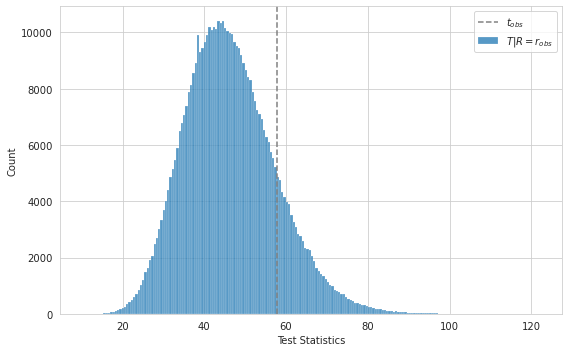
\includegraphics[width=0.55\textwidth]{midterm-1.png}
  \captionsetup{justification=centering}
\end{figure*}

\newpage
\section{Q9}
We prove the rule $\delta(x_{obs})$: "rejects $H_o: k = k^*$ if $p(x_{obs}|k^*) \le 2.5\%$" indeed has Type I error rate of $\alpha = 2.5\%$ at any $k^* > 0$ fixed.
\begin{align*}
    E[\delta(x_{obs}) = H_1|H_o:k=k^*] &= E[I(p(x_{obs}|k^* \le 2.5\%) | H_o] \\
        &= P(p(x_{obs}|k^*) \le 2.5\% | H_o) \\
        &= P(x_{obs} \le F^{-1}(2.5\%) | H_o) \\
        &= F(F^{-1}(2.5\%)) = 2.5\%
\end{align*}

\section{Q10}
Here we define the interval rule for $k$, where $F^{-1}(\cdot, k^*)$ is the quantile function of the conditional p-value $p(x_{obs}|k^*)$.
\begin{align*}
    \gamma(X) &= [\underline{\gamma}(X), \overline{\gamma}(X)] \\
    \overline{\gamma}(X) &= \mathop{\arg\max}_{k^*} F^{-1}(0.025, k^*) \\
    \underline{\gamma}(X) &= \mathop{\arg\min}_{k^*} F^{-1}(0.975, k^*)
\end{align*}
To claim $\gamma(X)$ is a 95\% confidence interval rule for the Negative Binomial model is ebulliently for us to show for any $x_{obs} \in \mathscr{X}$ the minimum coverage is 95\%. The confidence rule $\gamma$ requires a quantile estimation of the test statistics $T$'s distribution over all possible ranges of $k^*$ and $x_{obs}$, which I believe is analytically intractable. Hence, I brutal-forced a small region of the entire space to show an example for an engineer's proof. Mainly, I simulated many synthetic datasets through the Negative Binomial model so we know the ground truth. I used the composite sampling of Multinomial and Dirchilet to estimate the distribution of $T$, then estimated the interval $\gamma(x_{obs})$ using a discrete approximation of the quantile. The coverage is estimated across randomly sampled synthetic datasets with $\tau \thicksim U(0.0012, 0.05), \mu=100, n=36$. 

The below plot showcases the result after 2,530 Monte Carlo samples --- it is quite expensive to evaluate at each step. The mean Monte Carlo estimated coverage ratio is $93.20\% \pm 0.98\%$ with its 95th Monte Carlo estimated interval. 

\begin{figure*}[!h]
  \centering
  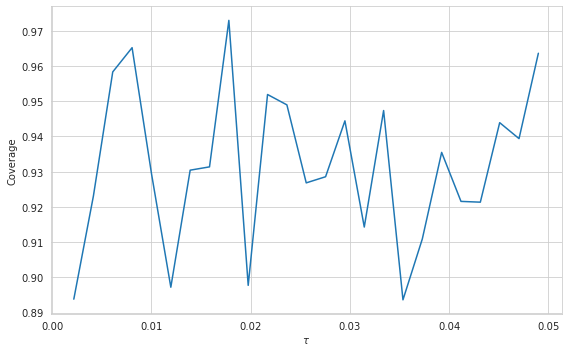
\includegraphics[width=0.55\textwidth]{midterm-2.png}
  \captionsetup{justification=centering}
\end{figure*}

\end{document}